% ********** Chapter 4 **********
\chapter{Case Studies}
\label{chapter6}

Along this chapter, the used case studies are explained in detail. In section \ref{chap6:overview}, an overview is given. Furthermore, in section \ref{chap6:alarm}, the Alarm System case study is presented, together with its results. Finally, in section \ref{chap6:stream}, the second case study, Input/Output Streams, is presented together with its results.

\section{Overview}
\label{chap6:overview}
The overall intention of this case studies is to show the capabilities of the mapper specified and presented in chapter \ref{chapter5}. The first example, the Alarm System, is intended to show the overall functionalities of the mapper. On the other hand, the Input/Output Streams case study is intended to show an example of how the mapper deals with multiple inheritance situations.


\section{Alarm System}
\label{chap6:alarm}

In this section, the Alarm System case study will be presented. This case study, which can be seen in detail in \cite{Fitzgerald&05}, is intended to test the overall functionalities of this mapper.

First, an introduction to the problem will be performed. There are three entities in this Alarm System of a chemical plant: the Expert, the Alarm and the Plant. In this alarm system, whenever an alarm is raised in a plant, an expert with the right qualifications is called to deal with situation. The implementation in \vpp\ of each entity is provided below.

\begin{description}
\item{\textbf{Expert}}
\lstset{style=mystyle}
\lstset{language=VDM++}
\begin{lstlisting}
class Expert

instance variables

quali : set of Qualification;

inv quali <> {};

types
public Qualification = 
     <Mech> | <Chem> | <Bio> | <Elec>;

operations
public Expert: set of Qualification 
             ==> Expert
Expert(qs) == quali := qs
pre qs <> {};

public GetQuali: () 
          ==> set of Qualification
GetQuali() == return quali;
  
end Expert
\end{lstlisting}
\item{\textbf{Alarm}}
\begin{lstlisting}
class Alarm

types

public String = seq of char;

instance variables 

descr    : String;
reqQuali : Expert`Qualification;

operations

public Alarm: Expert`Qualification * String ==> Alarm
Alarm(quali,str) ==
( descr := str;
  reqQuali := quali
);

public GetReqQuali: () ==> Expert`Qualification
GetReqQuali() ==
  return reqQuali;
  
end Alarm
\end{lstlisting}
\item{\textbf{Plant}}
\begin{lstlisting}
class Plant

instance variables

alarms   : set of Alarm;
schedule : map Period to set of Expert;
inv PlantInv(alarms,schedule);

functions

PlantInv: set of Alarm * map Period to set of Expert -> 
          bool
PlantInv(as,sch) ==
  (forall p in set dom sch & sch(p) <> {}) and
  (forall a in set as &
     forall p in set dom sch &
       exists expert in set sch(p) &
         a.GetReqQuali() in set expert.GetQuali());

types

public Period = token;
  
operations

public ExpertToPage: Alarm * Period ==> Expert
ExpertToPage(a, p) ==
  let expert in set schedule(p) be st
      a.GetReqQuali() in set expert.GetQuali()
  in
    return expert
pre a in set alarms and
    p in set dom schedule
post let expert = RESULT
     in
       expert in set schedule(p) and
       a.GetReqQuali() in set expert.GetQuali();
	 
public NumberOfExperts: Period ==> nat
NumberOfExperts(p) ==
  return card schedule(p)
pre p in set dom schedule;

public ExpertIsOnDuty: Expert ==> set of Period
ExpertIsOnDuty(ex) ==
  return {p | p in set dom schedule & 
              ex in set schedule(p)};

public Plant: set of Alarm * 
              map Period to set of Expert ==> Plant
Plant(als,sch) ==
( alarms := als;
  schedule := sch
)
pre PlantInv(als,sch);

end Plant
\end{lstlisting}
\end{description}

After running the mapper from \vpp\ to \jml, the following results are achieved:

\begin{description}
\item{\textbf{Expert}} The expert specification converted to \jml\ is as follows. The type presented is not being considered by the mapper, thus it has no correspondence.
\lstset{language=Java}
\lstset{style=JML}
\begin{lstlisting}
//@ model import org.jmlspecs.models.JMLValueSet;
import java.util.Set;

public class Expert{

	//@ public model JMLValueSet quali;
	
	/*@ public invariant
	  @   !quali.isEmpty();
	  @*/

	//@ requires !q.isEmpty();
	public Expert(Set q);
	
	public Set getQuali();

}
\end{lstlisting}

\item{\textbf{Alarm}} This class was mapped without loose of information (except methods bodies, which are not being considered).
\begin{lstlisting}

//@ model import org.jmlspecs.models.JMLString;
//@ model import org.jmlspecs.models.JMLEnumeration;

public class Alarm {

	//@ public model JMLString descr;
	//@ public model JMLEnumeration reqQuali;
	
	public Alarm(Enum reqQuali, String descr);
	
	public Enum getReqQuali();
}
\end{lstlisting}

\item{\textbf{Plant}} Finally, the plant class was mapped into \jml. Because it has a function, which is not being considered in this mapper, the function and where the function is being called has not been mapped. Thus, if one wants to have that specific function being mapped, the boolean expression of its body should be added inside, for example, the instance variables block, as an invariant.
\begin{lstlisting}
//@ model import org.jmlspecs.models.*;
import java.util.*;

public class Plant {

    //@ public model JMLValueSet alarms;
	//@ public model JMLValueToValueMap schedule;
	
	
	public Plant(Set s,HashMap m);
	
	/*@ public normal_behaviour
	  @
	  @ requires
	  @ this.alarms.contains(a) && 
	  @ this.schedule.containsKey(p);
	  @
	  @ ensures
	  @ ((Set) this.schedule.get(p)).contains(\result)
	  @ && 
	  @ \result.getQuali().contains(a.getReqQuali());
	  @ assignable this.alarms, this.schedule;
	  @*/
	public Expert expertToPage(Alarm a, Object p);
	

	public Set expertIsOnDuty(Expert p);

	/*@ public normal_behaviour
	  @ requires
	  @ (this.schedule.keySet()).contains(p);
	  @*/	
	public int numberOfExperts(Object p);
}
\end{lstlisting}
\end{description}

\lstset{language=VDM++}
\lstset{style=mystyle}

The results from this case study were correct, and the mapper showed no problems performing the translation. However, in the case of the Plant class, some constraints were not respected, thus the result is not quite what it was expected.

\section{Input/Output Streams}
\label{chap6:stream}

Along this section, it is possible to see an introduction to the case study, in subsection \ref{chap6:case2:intro}, which consists in a description of the problem and the motivation for using it. Furthermore, the specification of the classes can be found in subsection \ref{chap6:case2:spec} and finally in subsection \ref{chap6:case2:res}, the results of using the  bidirectional mapper with this case study are presented along with an analysis of those results.


\subsection{Introduction}
\label{chap6:case2:intro}

This case study consists in having \vpp\ classes that represents input/output streams. Streams are channels that allow programs to interact with the surrounding environment. This case study was chosen in order to have a multiple inheritance scenario tested by the pre-processor, which is explained in section \ref{chap5:preproc}, and by the mapper itself, explained in section \ref{chap5:mapper}. The referred multiple inheritance scenario, called \textit{diamond problem} in object-oriented languages, has to be resolved in order to map the case study from \vpp\ to \jml. 

There are four classes, specified in \vpp\ and presented in section \ref{chap6:case2:spec}, evolved in this case study: \textit{IO}, \textit{InputStream}, \textit{OutputStream} and \textit{IOStream}. Figure \ref{chap6:case2:diam} illustrates a simple class diagram containing those four classes and how they hand together.

\begin{figure}[!htb]
\begin{center}
\resizebox{.70\textwidth}{!}{\includegraphics{chap6/classdiag.ps}}
\end{center}
\caption{Illustration of the input/output stream case study.}
\label{chap6:case2:diam}
\end{figure}

As it can be seen from the class diagram, the class \textit{IO} is subclass of both \textit{InputStream} and \textit{OutputStream} classes. Furthermore, the class \textit{IOStream} is subclass of both \textit{InputStream} and \textit{OutputStream} classes. Thus, a multiple inheritance problem arises from this last fact. Note that the methods are not implemented in all the classes and there are no specifications (e.g., pre-conditions) in any of the classes, because the goal of this case study is to verify how the multiple inheritance issue is solved when moving from \vpp\ to \jml.

It is expected, using the mapper from \vpp\ to \jml, that the multiple inheritance issue is detected and resolved by the pre-processor, and also that the mapper will be able to generate the \jml\ representation of these classes.


\subsection{Specification}
\label{chap6:case2:spec}


As it was said in section \ref{chap6:case2:intro}, this case study is composed by four classes specified in \vpp\. In this section, the four classes are presented together with a description of each one.

\begin{description}

\item{\textbf{IO}} The following class is the superclass of both \textit{InputStream} and \textit{OutputStream} classes. It defines the skeleton of any class who implements a stream. The specification of this class can be foune below.

\lstset{style=mystyle}
\bigskip
\begin{lstlisting}
class IO

types

public byte = nat;

operations 

public read : seq of byte  ==> nat
read(b) == is subclass responsibility;

public write : seq of byte  ==> ()
write(b) == is subclass responsibility;

public close : () ==> ()
close() == is subclass responsibility;

end IO
\end{lstlisting}
\bigskip

\item{\textbf{InputStream}} This class is a subclass of the \textit{IO} class, which represents an input stream. Below, one can find the specification of this class.

\bigskip
\begin{lstlisting}
class InputStream is subclass of IO

operations

public read : seq of byte ==> nat
read(b) == is not yet specified;

public close : () ==> ()
close() == is not yet specified;


end InputStream
\end{lstlisting}
\bigskip

\item{\textbf{OutputStream}} This class represents an output stream, and its a subclass of the class \textit{IO}, presented above. The specification of this class can be found below.

\bigskip
\begin{lstlisting}
class OutputStream is subclass of IO

operations

public write : seq of byte ==> ()
write(b) == is not yet specified;

public close : () ==> ()
close() == is not yet specified;

end OutputStream
\end{lstlisting}
\bigskip

\item{\textbf{IOStream}} Finally, this class represents a bidirectional stream, both for input and output. It inherits both from the \textit{InputStream} and \textit{OutputStream}, thus this class enforces a multiple inheritance scenario. It contains three methods: \textit{read}, \textit{write} and \textit{close}. The specification of this class is shown below.

\bigskip
\begin{lstlisting}
class IOStream is subclass of InputStream, OutputStream

operations

public read : seq of byte ==> nat
read(b) == is not yet specified;

public write : seq of byte  ==> ()
write(b) == is not yet specified;

public close : () ==> ()
close() == is not yet specified;

end IOStream
\end{lstlisting}
\bigskip

\end{description}


\subsection{Results}
\label{chap6:case2:res}

As it was said in section \ref{chap6:case2:intro}, the main goal of this case study is to verify how the mapper deals with multiple inheritance situations. Thus, an explanation will be presented below concerning the steps of the pre-processor with respect to these specifications.

The pre-processor will start by checking if there are multiple inheritance within the specification.  The main operation \textit{init} presented in chapter \ref{chapter5} will call the operation \textit{preprocess}, which will perform such test. The operation is listed below.

\bigskip
\begin{lstlisting}
public preprocess : 
  OmlSpecifications ==>
  bool
preprocess(specs) == 
  let l = specs.getClassList()
  in return hasMultipleInheritance(l);
\end{lstlisting}
\bigskip

In this case, after executing the \textit{preprocess} operation, the VDMTools interpreter will return the following result:

\lstset{style=Example}
\bigskip
\begin{lstlisting}
>> p m1.preprocess(v.diamondproblem)
true
\end{lstlisting}
\bigskip

The operation returned the \textit{true} value, which means that at least one of the classes has multiple inheritance. At this point, the main operation \textit{init} will try to overcome the multiple inheritance problem by invoking the operation \textit{eliminateMI}. That operation is listed below.

\lstset{style=mystyle}
\bigskip
\begin{lstlisting}
public eliminateMI : 
  OmlSpecifications ==>
  JmlSpecifications
eliminateMI(specs) == 
  if canProceed(specs)
  then (eliminate(specs);
        build_jml(specs))
  else return new JmlSpecifications([]);
\end{lstlisting}
\bigskip

As it can be seen from the specification, the first test being performed is if it is possible proceed, \ie, if the multiple inheritance can be overcome. The operation responsible for such test is called \textit{canProceed} and it is shown below.

\bigskip
\begin{lstlisting}
public canProceed : 
  OmlSpecifications ==>
  bool
canProceed(specs) == 
  let cl = specs.getClassList(),
      s  = gatherInfo(cl)
  in result(s);
\end{lstlisting}
\bigskip

After executing that particular operation, the results from the VDMTools interpreter are as follows:

\lstset{style=Example}
\bigskip
\begin{lstlisting}
>> p m1.canProceed(v.diamondproblem)
true
\end{lstlisting}
\bigskip

Again, the result was positive, \ie, it is possible to eliminate the multiple inheritance issue. Thus, there is at most one class in the inheritance list that can remain a class, and all the other can be promoted to interfaces. In the case of this case study, the two classes in the inheritance list, \textit{InputStream} and \textit{OutputStream} can be promoted to interfaces. 

After that, the operation \textit{eliminateMI} can proceed with the elimination of the multiple inheritance. This elimination is gathering the information of which classes can be promoted to interfaces and which classes must remain classes. Furthermore, the \jml\ ASTs are built from the \vpp\ ASTs, and the result is an list of \jml\ classes. Because there is no pretty-printer available yet, the result cannot be shown . However, after generating the \jml\ classes, it is possible to see the state of the inheritance clauses of the \jml\ class \textit{IOStream}, which is the only one that had multiple inheritance at the \vpp\ level.

The results are as follows:

\lstset{style=Example}
\bigskip
\begin{lstlisting}
>> p let jml = m1.init(v.diamondproblem) 
     in jml.getClassList()(4).getClassVal().getInterfaceInheritance()
objref2742(JmlInterfaceInheritanceClause):
  < IJmlNode`ivColumn = 0,
    IJmlNode`ivInfo = { |-> },
    IJmlNode`ivLine = 0,
    JmlInterfaceInheritanceClause`ivIdentifierList = [ "InputStream",
      "OutputStream" ] >
\end{lstlisting}
\bigskip


From the execution shown above, one can see that the interface list of the class \textit{IOStream} is composed by the two classes that were superclasses at the \vpp\ level. Concerning the class inheritance list, its empty as it can be seen from the execution below:
\bigskip
\begin{lstlisting}
>> p let jml = m1.init(v.diamondproblem) 
     in jml.getClassList()(4).getClassVal().getInheritanceClause()
nil
\end{lstlisting}
\bigskip

Thus, the pre-processor together with the mapper had successfully eliminate the multiple inheritance issue present at the \vpp\ level and had generated correctly \jml\ classes. However, without a pretty-printer of the \jml\ AST, it is a hard task to analyse the results returned by the VDMTools interpreter. Thus, it is recommended as a future work to develop this component in order to see the results in a more readable perspective. 

Using the mapper on the other way arround, \ie, from \jml\ to \vpp, the same \vpp\ representation was achieved, this the results are not shown, due to the fact that they are identical to the initial classes.

% ********** End of chapter **********
